% Based on the "sig-alternate.tex" V2.1 April 2013
% This file should be compiled with V2.5 of "sig-alternate.cls" May 2012
% For tracking purposes - this is V2.0 - May 2012

\documentclass{sig-alternate-05-2015}


\begin{document}

% Copyright
\setcopyright{acmcopyright}
%\setcopyright{acmlicensed}
%\setcopyright{rightsretained}
%\setcopyright{usgov}
%\setcopyright{usgovmixed}
%\setcopyright{cagov}
%\setcopyright{cagovmixed}


% DOI
%\doi{10.475/123_4}

% ISBN
%\isbn{123-4567-24-567/08/06}

%Conference
\conferenceinfo{WWW}{2017 Perth, Western Australia, Australia}

\acmPrice{\$15.00}

%
% --- Author Metadata here ---
\conferenceinfo{WWW}{2017 Perth, Western Australia, Australia}
%\CopyrightYear{2007} % Allows default copyright year (20XX) to be over-ridden - IF NEED BE.
%\crdata{0-12345-67-8/90/01}  % Allows default copyright data (0-89791-88-6/97/05) to be over-ridden - IF NEED BE.
% --- End of Author Metadata ---

\title{Enhancing General Hypertext Editors with Automatic Supplemental Content Suggestions using a Semantic Knowledge Graph
\titlenote{A full version of this paper is available at
\texttt{TODO: Ephox/personal URL}}}
%
\numberofauthors{3} % REQUIRED for 3-column layout.
%
\author{
% 1st. author
\alignauthor
David Hyland-Wood\\
       \affaddr{Ephox Corporation}\\
       \affaddr{225 Montague Road, Level 4}\\
       \affaddr{West End, Queensland, Australia}\\
       \email{david.wood@ephox.com}
% 2nd. author
\alignauthor
Anna Harrison\\
       \affaddr{Ephox Corporation}\\
       \affaddr{225 Montague Road, Level 4}\\
       \affaddr{West End, Queensland, Australia}\\
       \email{anna.harrison@ephox.com}
% 3rd. author
\alignauthor
Ben Kolera\\
       \affaddr{Ephox Corporation}\\
       \affaddr{225 Montague Road, Level 4}\\
       \affaddr{West End, Queensland, Australia}\\
       \email{ben.kolera@ephox.com}
}

\maketitle
\begin{abstract}
Many types of writing, such as blog posts and business documents, could benefit from supplemental explanatory material to provide context, background, and additional information for exploration. The World Wide Web provides huge quantities of such supplementary material, but it is not generally suitable for inclusion in new writing due to issues of licensing, copyright, formatting, or syntax. Exceptions include clearly identifiable content meant to be embedded in hypertext documents, such as YouTube videos, and Twitter feeds. We demonstrate how the textual content in a general purpose hypertext editor may be used to automatically identify relevant supplementary material via artificial intelligence (AI) processes, and that material may be presented to a document author for possible inclusion in whole or in part. User interface elements are provided to allow an author to refine content suggestions with a minimum of input.
\end{abstract}


%
% The code below should be generated by the tool at
% http://dl.acm.org/ccs.cfm
% Please copy and paste the code instead of the example below. 
%
\begin{CCSXML}
<ccs2012>
<concept>
<concept_id>10010147.10010178.10010187.10010188</concept_id>
<concept_desc>Computing methodologies~Semantic networks</concept_desc>
<concept_significance>500</concept_significance>
</concept>
<concept>
<concept_id>10003120.10003123.10011759</concept_id>
<concept_desc>Human-centered computing~Empirical studies in interaction design</concept_desc>
<concept_significance>500</concept_significance>
</concept>
<concept>
<concept_id>10003456.10003457.10003567.10010990</concept_id>
<concept_desc>Social and professional topics~Socio-technical systems</concept_desc>
<concept_significance>300</concept_significance>
</concept>
<concept>
<concept_id>10010405.10010497.10010510.10010920</concept_id>
<concept_desc>Applied computing~Hypertext / hypermedia creation</concept_desc>
<concept_significance>300</concept_significance>
</concept>
</ccs2012>
\end{CCSXML}

\ccsdesc[500]{Computing methodologies~Semantic networks}
\ccsdesc[500]{Human-centered computing~Empirical studies in interaction design}
\ccsdesc[300]{Social and professional topics~Socio-technical systems}
\ccsdesc[300]{Applied computing~Hypertext / hypermedia creation}


%
% End generated code
%

%
%  Use this command to print the description
%
\printccsdesc

% We no longer use \terms command
%\terms{Theory}

\keywords{ACM proceedings; RDF; knowledge graph; Linked Data; IBM Watson}

\section{Introduction}
Many types of writing, such as blog posts and business documents, could benefit from supplemental explanatory material to provide context, background, and additional information for exploration. The World Wide Web provides huge quantities of such supplementary material, but it is not generally suitable for inclusion in new writing due to issues of licensing, copyright, formatting, or syntax. Exceptions include clearly identifiable content meant to be embedded in hypertext documents, such as YouTube videos, and Twitter feeds.

We wanted to determine whether the textual content in a general purpose hypertext editor may be used to automatically identify relevant supplementary material via artificial intelligence (AI) processes, and whether that material may be presented to a document author for possible inclusion in a document in a useful manner.

The techniques necessary for such an exploration are now generally available. Linguistic parsing of text content may be conducted relatively easily using generally available tools, at least in many European languages including English. Concept identification from the results of linguistic parsing has been similarly successful.

Concepts may be matched to relevant additional information by querying a graph of information in the Resource Description Framework (RDF) data model\cite{cyganiak2014rdf}. Such information form ``knowledge graphs" of related information. The first general purpose knowledge graph of scale was Freebase\cite{bollacker2008freebase}, which became the basis for the Google Knowledge Graph\cite{singhalintroducing}. Web search engines such as Google, Bing, and Yandex now use knowledge graphs to provide summaries of relevant information related to search terms. It is exactly this functionality that we wanted to add to our general purpose hypertext editors.

\section{Architecture}

\begin{figure*}
\centering
%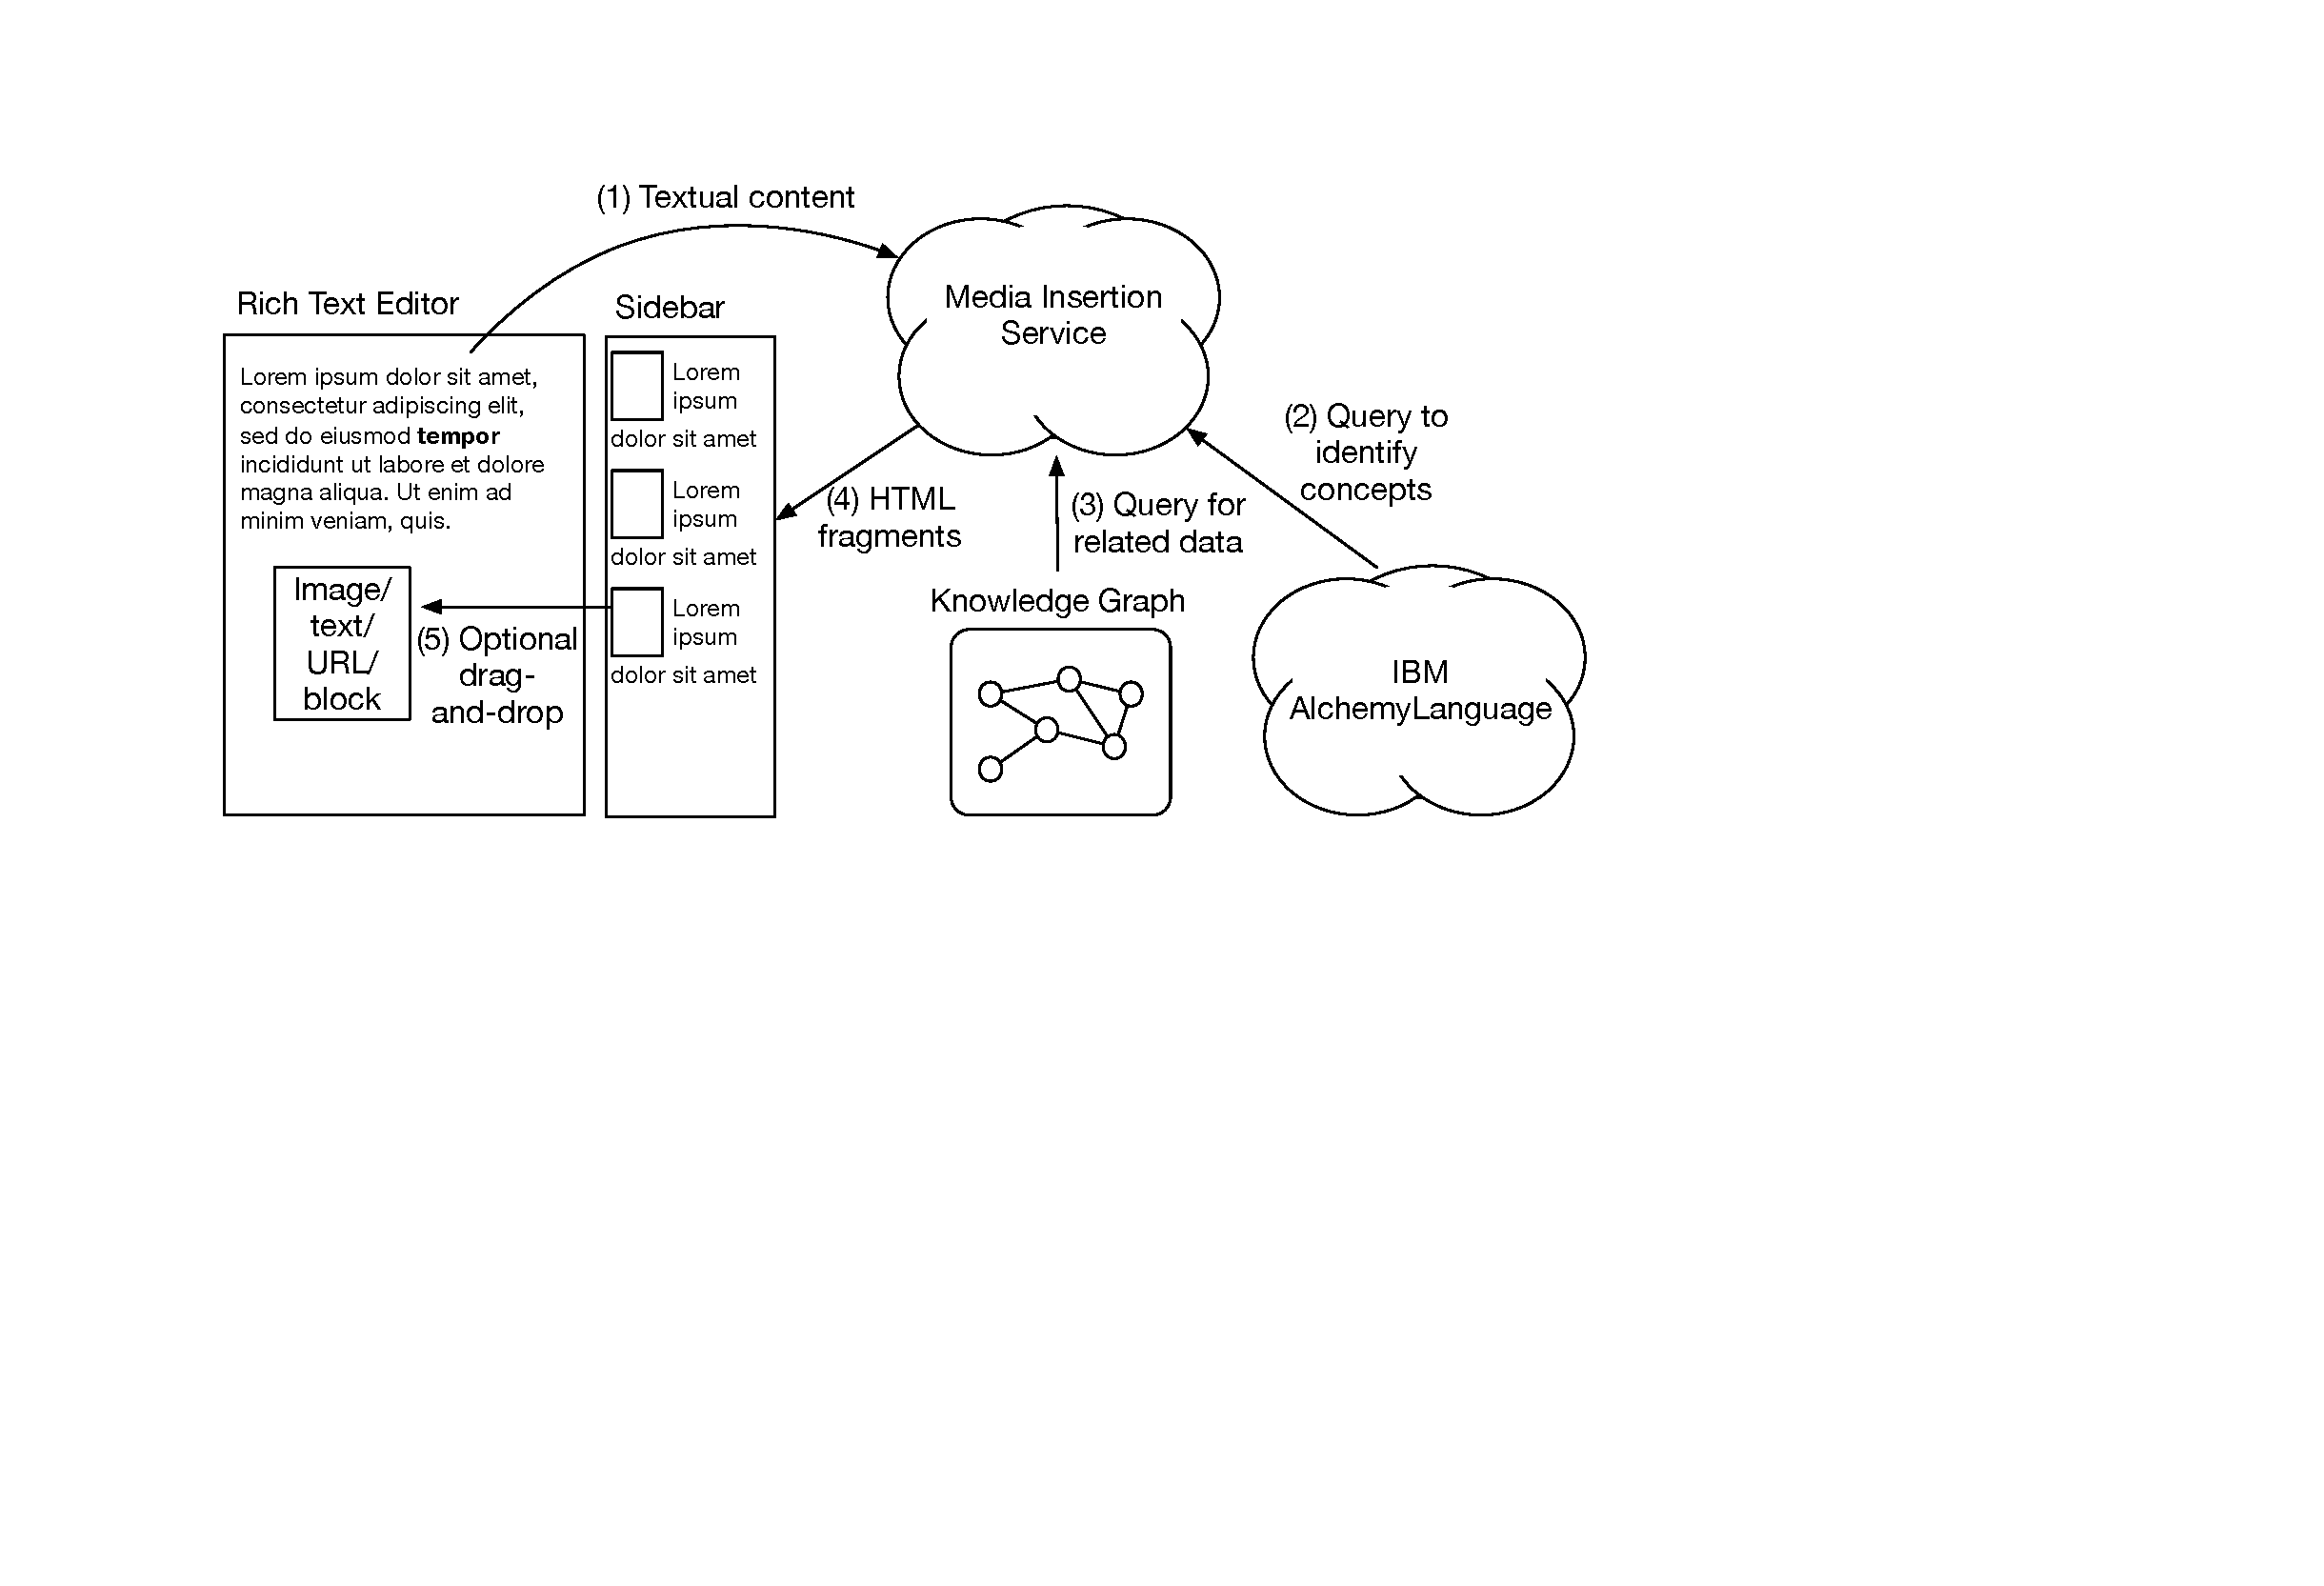
\includegraphics[height=1in, width=1in]{KGarchitecture}
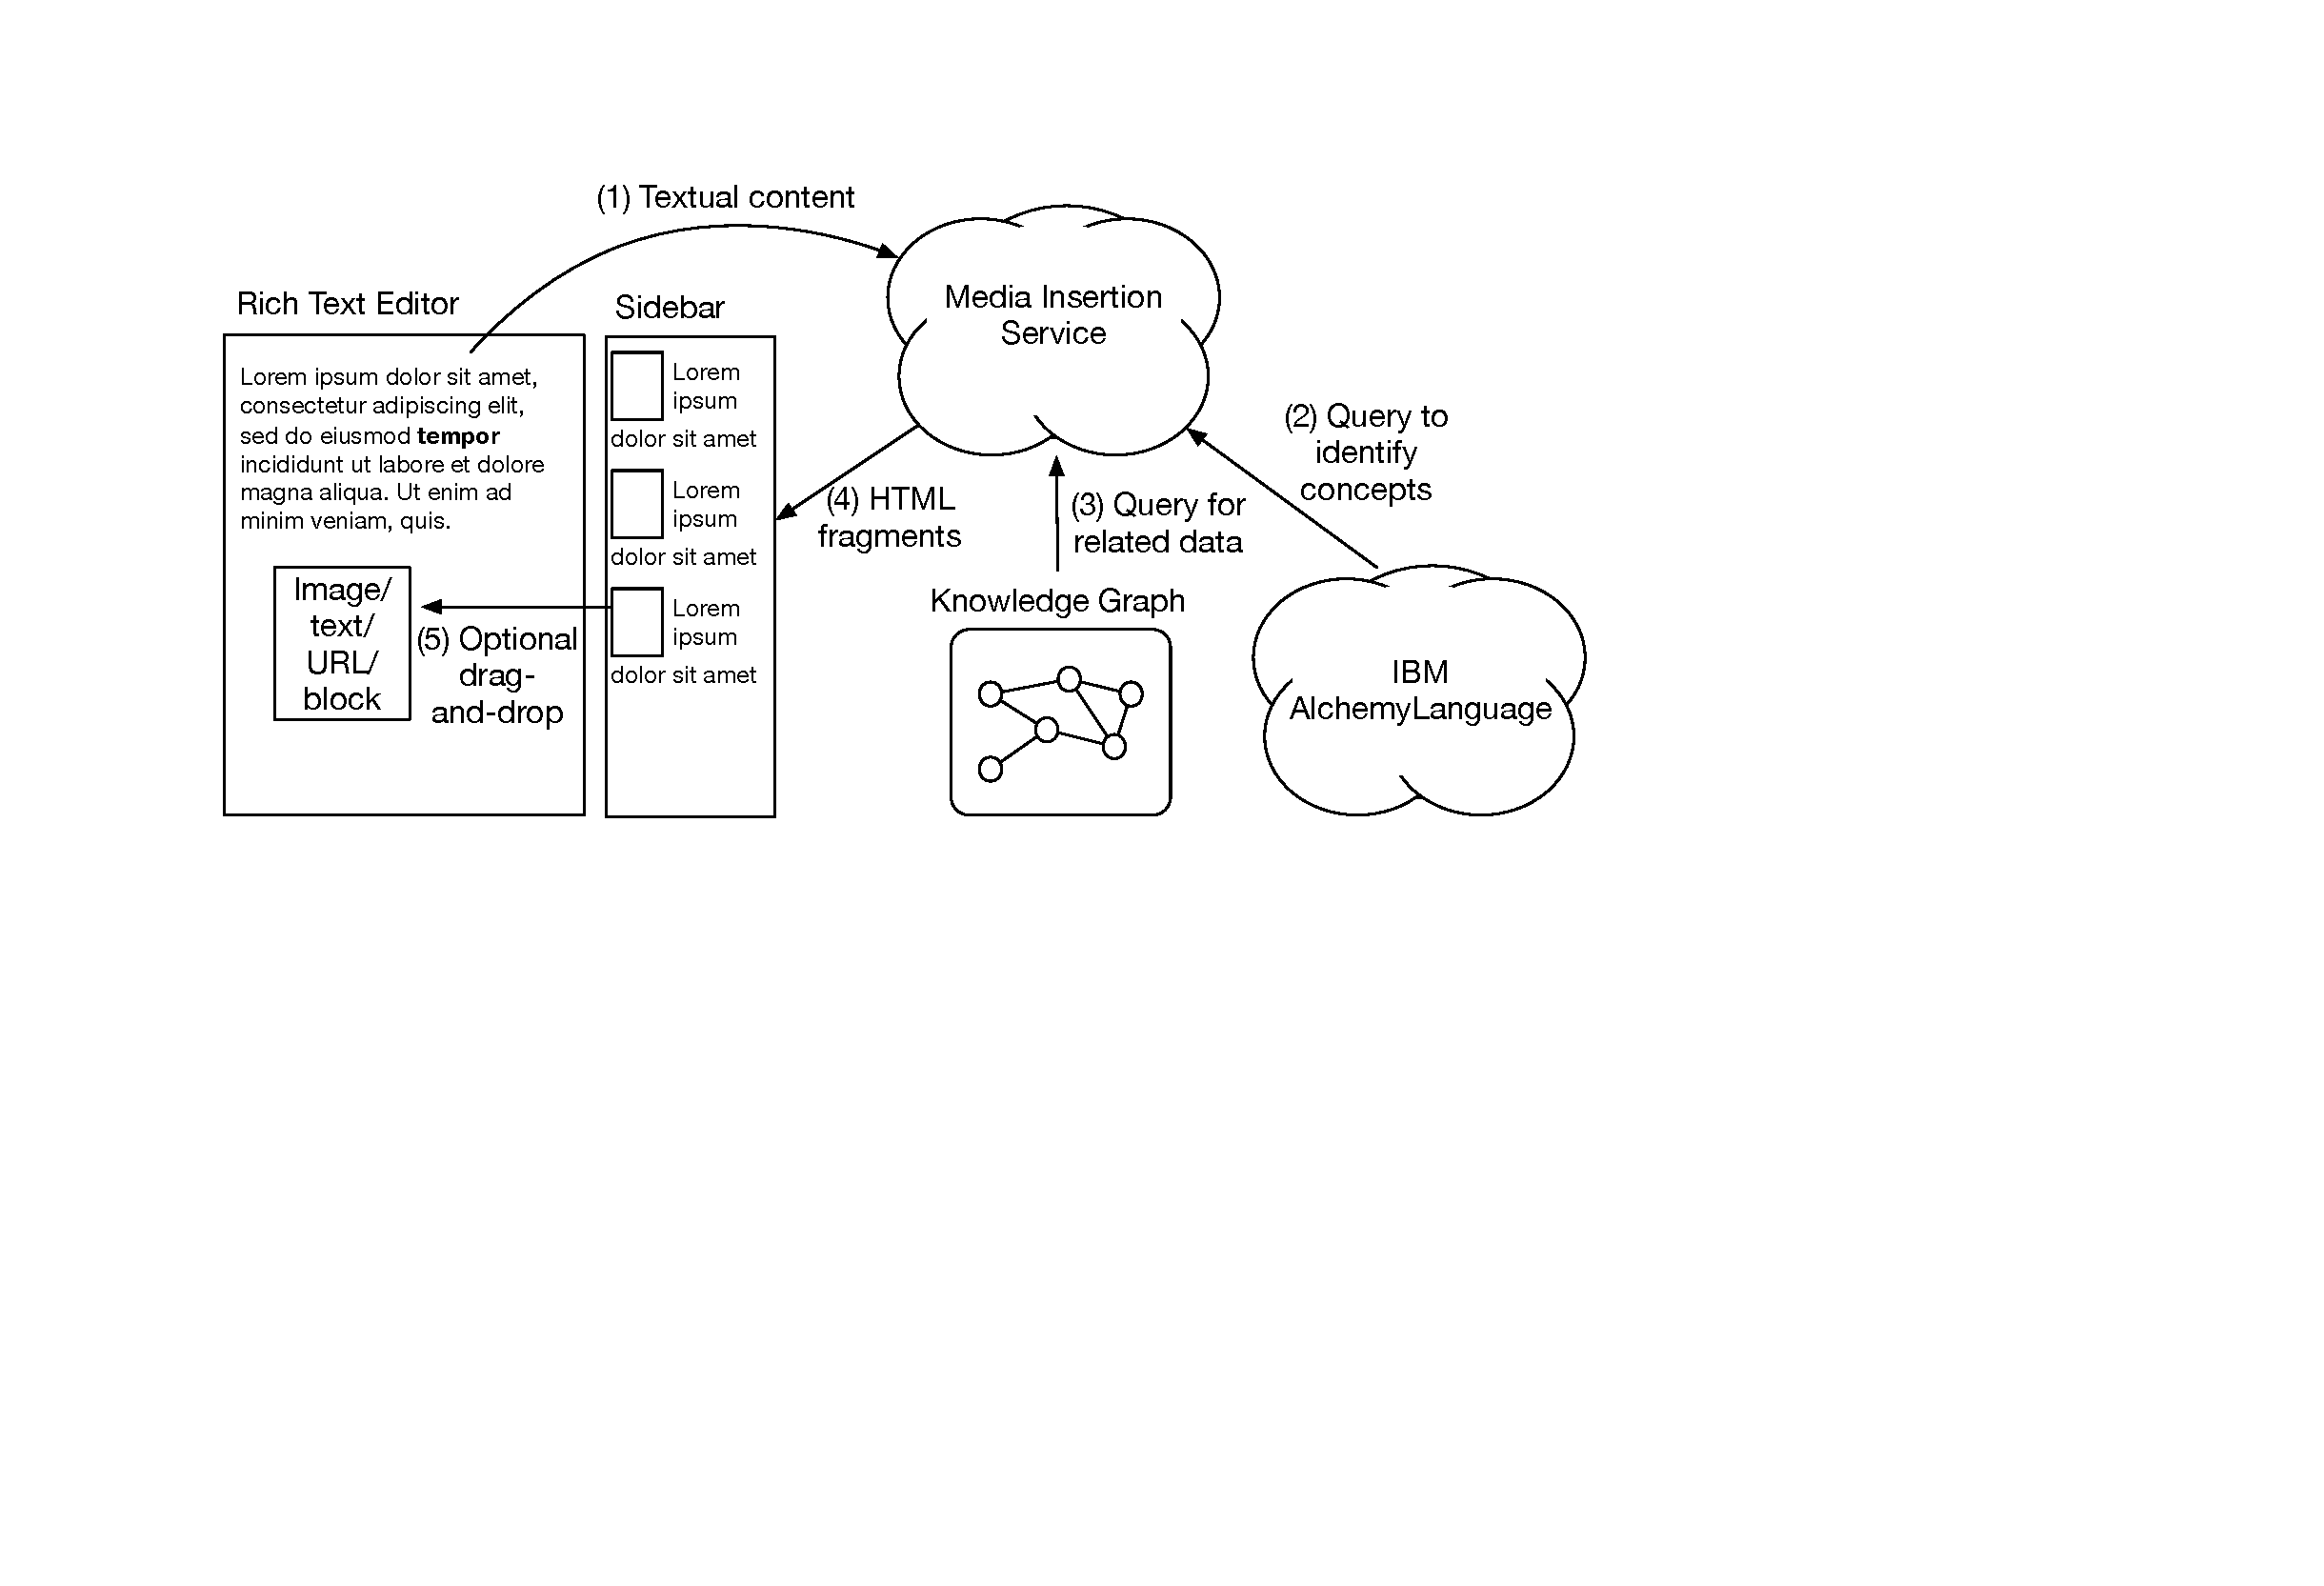
\includegraphics[scale=0.6]{KGarchitecture}
\caption{Data flow from editor to sidebar via enhancement services.}
%\vskip -6pt
\end{figure*}

We wrapped one of our JavaScript hypertext editors, Textbox.io, to include a sidebar for the presentation of supplemental material. The sidebar is a simple HTML component that accepts HTML fragments for display and possible drag-and-drop of components into the editor's content pane. JavaScript is used to query on online service to search for relevant information based upon the current contents of the editor.

Textual content is written into the editor by a document author. That content is uploaded to an Ephox cloud service for analysis (Figure 1). The Ephox service sends the content to another service to parse the content, and extract concepts. We used IBM's online AlchemyLanguage service\footnote{\texttt{http://www.alchemyapi.com/products/alchemylanguage/}} for linguistic parsing and concept identification, although any number of similar services could have been used for those purposes. AlchemyLanguage is based upon IBM's Watson question-answering AI system\cite{ferrucci2010building}. One advantage of the AlchemyLanguage API is that its concept tagging service\footnote{\texttt{http://www.alchemyapi.com/products/alchemylanguage/\allowbreak{}concept-tagging}} returns DBpedia\cite{auer2007dbpedia} URIs for each identified concept.

DBpedia URIs conveniently serve as indexes into an RDF knowledge graph. To implement the knowledge graph service, we used an Apache Tomcat\footnote{\texttt{https://tomcat.apache.org/}} Web application server with a RDF4J\footnote{\texttt{http://rdf4j.org/}} version 2.0 RDF database engine. Relevant portions of DBpedia were sharded into six RDF4J databases to speed both data indexing and assist query performance. DBpedia topical concepts, SKOS\cite{miles2009skos} categories, labels, image URLs, short abstracts, categories and their labels, transitive instance types, mapping-based objects and literals, and person data were used for our initial experiments. We limited our DBpedia extracts to the English language due to the language limitations of the AlchemyLanguage concept tagging service.

Two SPARQL 1.1\cite{harris2013sparql} queries against the knowledge graph were used to construct supplemental material representations:

\begin{itemize}
\item The first SPARQL query is used to identify the type of a concept (i.e. each concept will be either a person, place, organization, movie, species, product, or a general concept).
\item The second SPARQL query is used to identify available data about a specific concept, as anticipated by its type.
\end{itemize}

Thus, a concept of type ``person" might have a birth date and a birth place. A place might have area and a population estimate, etc. Most data elements for any given type are considered to be optional.

The results of the second query are used to fill a type-specific HTML template. An HTML fragment is produced for each concept, and any empty divs are removed. The completed fragment is returned to the editor's sidebar for display.

SPARQL 1.1 SERVICE clauses were used to execute federated queries\cite{prud2013sparql} across the various databases making up the knowledge graph.

We chose to construct our own knowledge graph instead of using one provided by the AlchemyLanguage service. We wish to eventually refine and contextualize the contents of the knowledge graph over time to provide industry- or even customer-specific data. We also wanted to be able to swap linguistic parsing and concept tagging services if desired at a later time.

\section{Usage}

\textbf{TODO:} Anna? How did people approach the sidebar? How did they use it? Did anything unexpected happen during use?

\textbf{TODO:} User interface elements are provided to allow an author to refine content suggestions with a minimum of input.

\section{Evaluation}

\textbf{TODO:} Anna to conduct user testing to determine an objective basis for the value provided.

\section{Conclusions and Further Work}
We have demonstrated that the automatic suggestion of reuseable supplementary information in a general purpose hypertext editor can assist authors to create content. The combination of linguistic parsing, concept extraction, knowledge graph query, and contextual templating were effective techniques to provide such supplementary material. \textbf{TODO:} Confirm based on Anna's results.

Interface testing of content authors showed that... \textbf{TODO:} (e.g. Adding a KG helps users to create supplemental content more rapidly, or adding a KG helps avoid content recreation by linking and reusing existing resources.)

Our immediate next step is to productize the server-side portion of our work. We intend to deploy knowledge graph services in several Amazon Web Services availability zones to facilitate rapid network access in geographical regions where our largest customers are located. We will also add the client-side portion into production versions of our JavaScript rich text editors, Textbox.io and TinyMCE.

We intend to increase the number of concept types, and their associated templates.

We intend to grow the size and complexity of the Ephox knowledge graph beyond general encyclopaedic content in order to present supplementary material in progressively more contextual ways. We would like to include data that is specific to particular industries, such as manufacturing or pharmaceutical content, and even allow for extension by customers to allow querying of company-specific data. Finally, we intend to extend our user interface to link the presented concepts to related concepts, so that a user will be able to explore relevant content within the editing environment.
%\end{document}  % This is where a 'short' article might terminate

%ACKNOWLEDGMENTS are optional
\section{Acknowledgments}
The authors would like to thank James Johnson for prototyping IBM Watson integration into Ephox editors, and Ephox Corporation for supporting this work.

%
% The following two commands are all you need in the
% initial runs of your .tex file to
% produce the bibliography for the citations in your paper.
\bibliographystyle{abbrv}
\bibliography{bibliography}  % sigproc.bib is the name of the Bibliography in this case
% You must have a proper ".bib" file
%  and remember to run:
% latex bibtex latex latex
% to resolve all references
%
% ACM needs 'a single self-contained file'!

%\balancecolumns % GM June 2007
% That's all folks!
\end{document}
